% pdflatex solver.tex
\documentclass[11pt]{article}

\usepackage[margin=1in]{geometry}
\usepackage{amsmath,amssymb}
\usepackage{booktabs}
\usepackage{listings}
\usepackage{pgfplots}
\pgfplotsset{
  compat=1.18,
  solveraxis/.style={
    width=0.86\textwidth,
    scale only axis,
    tick label style={font=\small},
    label style={font=\small},
    legend cell align=left,
    legend style={font=\small, draw=none},
  },
}
\tikzset{
  upwind/.style={thick, draw=blue!60!black},
  welge/.style={thick, dashed, draw=red!70!black},
  declare function={
    sn(\t)=(\t-0.2)/0.6;
    lw(\t)=(sn(\t))^2;
    lo(\t)=0.5*(1-sn(\t))^2;
    ff(\t)=lw(\t)/(lw(\t)+lo(\t));
    hull(\t)=ifthenelse(\t<=0.54641,2.27671*(\t-0.2),ff(\t));
  },
}
\usepackage[hidelinks]{hyperref}

\lstset{
  basicstyle=\ttfamily\small,
  columns=fullflexible,
  breaklines=true,
  frame=single,
  framerule=0.3pt
}

\title{Solving the 1D Buckley--Leverett problem\\ with AMGCL}
\author{1D Buckley--Leverett notes}
\date{}

\begin{document}
\maketitle

\begin{abstract}
This note describes the sequential implicit program in \texttt{src/buckley\_leverett.cpp}.
Saturation is advanced by implicit upwind Newton iterations.
Pressure is a two-point flux discretization of the total-velocity equation.
Both linear systems are solved by AMGCL~1.4.3.
The derivation of $f(S)$, the Welge tangent, and the bidiagonal Jacobian is in \texttt{theory.tex}.
\end{abstract}

\section{What is integrated}

The unknowns are the cell water saturation $S_i$ and the cell pressure $p_i$ on $x\in[0,1]$.
Time is in pore volumes injected.
The equations are
\begin{equation}
\label{eq:pde}
\frac{\partial S}{\partial t} + \frac{\partial f(S)}{\partial x} = 0,
\qquad
\frac{d}{dx}\!\left(k(x)\,\lambda_t(S)\frac{dp}{dx}\right) = 0,
\end{equation}
with the rate boundary condition and the outlet pressure
\begin{equation}
\label{eq:p-bc}
-k\lambda_t\frac{dp}{dx} = 1,
\qquad
p(1) = 0.
\end{equation}
Corey data are $S_{wc}=S_{or}=0.2$, $n_w=n_o=2$, $k_{rw}^{0}=k_{ro}^{0}=1$, $\mu_w=1$, $\mu_o=2$, so the endpoint mobility ratio is $M=2$.
Absolute permeability is dimensionless and piecewise constant:
\begin{equation}
\label{eq:k}
k(x) =
\begin{cases}
0.1, & 0.45 \le x < 0.55,\\
1, & \text{otherwise.}
\end{cases}
\end{equation}
The streak steepens $dp/dx$.
It does not change $S$.
In one dimension, incompressible flow with only an inlet and an outlet has $\partial u_t/\partial x = 0$, and the inlet rate fixes $u_t = 1$.
Fractional flow does not depend on $k$.

The initial saturation is $S_{wc}$ in every cell.
Cell centers are $x_i = (i+\tfrac12)\Delta x$.

\section{One time step}

The target step is limited by the shock CFL,
\begin{equation}
\label{eq:cfl}
\Delta t = \mathrm{CFL}\,\frac{\Delta x}{v_s},
\end{equation}
with default $\mathrm{CFL}=1$.
The default final time is $t = 0.55/v_s$, which places the Welge shock at $x=0.55$.
Both defaults can be overridden by
\begin{lstlisting}
buckley [cells] [pore_volumes] [cfl]
\end{lstlisting}
The loop is sequential, sometimes called sequential implicit for the saturation part:
\begin{enumerate}
\item Given $S^n$, solve the nonlinear saturation step for $S^{n+1}$ at the fixed total velocity $1$.
Newton's matrix changes at every iteration and is solved with BiCGStab and algebraic multigrid.
\item Given $S^{n+1}$, assemble and solve the linear pressure system with CG and algebraic multigrid.
The pressure is a diagnostic in this configuration: the saturation update does not read it, because the rate is already known.
The solve is still checked, because the discrete face fluxes must reproduce the boundary rate.
\item Advance time and add the outlet water volume $f(S_{N-1}^{n+1})\,\Delta t$.
\end{enumerate}
If Newton or the linear solver fails, $\Delta t$ is halved, up to twelve times, and the step is repeated from $S^n$.
The default $800$-cell run does not cut the step.

\section{Saturation: Newton on the upwind residual}

The residual and its Jacobian are derived in \texttt{theory.tex}.
In code they are \texttt{residual\_linf} and \texttt{assemble\_transport}.
With $a = \Delta x/\Delta t$ and with the inlet flux equal to $1$,
\begin{equation}
\label{eq:R}
R_i = a\,(S_i - S_i^n) + f(S_i) - f_{\mathrm{up},i},
\qquad
f_{\mathrm{up},0} = 1,
\quad
f_{\mathrm{up},i} = f(S_{i-1}).
\end{equation}
The nonzero Jacobian entries are
\begin{equation}
\label{eq:J}
J_{i,i} = a + f'(S_i),
\qquad
J_{i,i-1} = -f'(S_{i-1})\ (i\ge 1).
\end{equation}
Column indices are stored in increasing order in a CRS triple $(\mathtt{ptr}, \mathtt{col}, \mathtt{val})$.
The Newton right-hand side is $-R$.

Each Newton iteration stops when $\|R\|_\infty < 10^{-9}$, and gives up after $15$ iterations.
The update is damped if a full step does not decrease the residual: the trial saturation is
\[
S_i \leftarrow \mathrm{clamp}\bigl(S_i + \omega\,\delta_i,\, S_{wc},\, S_{\max}\bigr),
\]
and $\omega$ starts at $1$ and is halved until the infinity norm of $R$ does not increase.
Clamping keeps the relative permeabilities inside the Corey interval.

$f$ and $f'$ are analytic.
\texttt{Fluid::flow} evaluates~\eqref{eq:J}'s derivative from the quotient rule on $\lambda_w(S)$ and $\lambda_o(S)$, including the factor $ds/dS$.
A startup check compares that derivative with a centered difference on $(S_{wc}, S_{\max})$ and requires an error below $10^{-5}$.
The default data give about $1.7\times 10^{-10}$.

\section{Pressure: two-point flux}

Mobility is frozen at the saturation just accepted, and $k$ is the cell value~\eqref{eq:k}.
The half-transmissibility from a cell center to a face a distance $\Delta x/2$ away is
\begin{equation}
\label{eq:half}
T_i^{\mathrm{half}} = \frac{2 k_i \lambda_t(S_i)}{\Delta x}.
\end{equation}
The face transmissibility is the harmonic mean of the two half-transmissibilities,
\begin{equation}
\label{eq:face}
T_{i+1/2}
=
\frac{T_i^{\mathrm{half}}\, T_{i+1}^{\mathrm{half}}}{T_i^{\mathrm{half}} + T_{i+1}^{\mathrm{half}}}.
\end{equation}
Finite-volume statements of~\eqref{eq:p-bc}, with the outlet face held at $p=0$, are
\begin{equation}
\label{eq:tpfa}
\begin{aligned}
T_{1/2}(p_0 - p_1) &= 1,\\
T_{i-1/2}(p_i - p_{i-1}) + T_{i+1/2}(p_i - p_{i+1}) &= 0,\\
T_{N-3/2}(p_{N-1} - p_{N-2}) + T_{N-1}^{\mathrm{half}}\, p_{N-1} &= 0.
\end{aligned}
\end{equation}
The matrix is symmetric, with positive diagonal and nonpositive off-diagonal entries.
The outlet Dirichlet condition removes the constant-pressure null space, so the matrix is symmetric positive definite and CG is appropriate.
Because $k\lambda_t$ is cellwise constant, the exact solution of~\eqref{eq:tpfa} is the recurrence
\begin{equation}
\label{eq:p-exact}
p_{N-1} = 1/T_{N-1}^{\mathrm{half}},
\qquad
p_i = p_{i+1} + 1/T_{i+1/2},
\end{equation}
which is also the integral of $dp = -dx/(k\lambda_t)$ from cell center to cell center.
The AMGCL pressure is compared with~\eqref{eq:p-exact}, and every face flux $T(p_i-p_{i+1})$ is compared with $1$.
Both discrepancies are about $10^{-11}$ on the default run.
This tests the linear solver, not a further modeling error: the discrete system is integrated exactly by~\eqref{eq:p-exact}.

\section{Where AMGCL is called}

AMGCL is a header-only algebraic multigrid library.
The program uses the compile-time interface and defines \texttt{AMGCL\_NO\_BOOST}, so Boost is not required.
The builtin backend stores the matrix in CRS.
The adapter \texttt{amgcl/adapter/crs\_tuple.hpp} accepts the system as
\begin{lstlisting}
std::tie(n, ptr, col, val)
\end{lstlisting}
with \texttt{n} and the three arrays passed as non-const lvalues.
The two solver types are
\begin{lstlisting}
using Backend = amgcl::backend::builtin<double>;

using PressureSolver = amgcl::make_solver<
    amgcl::amg<Backend,
        amgcl::coarsening::smoothed_aggregation,
        amgcl::relaxation::spai0>,
    amgcl::solver::cg<Backend>>;

using TransportSolver = amgcl::make_solver<
    amgcl::amg<Backend,
        amgcl::coarsening::smoothed_aggregation,
        amgcl::relaxation::ilu0>,
    amgcl::solver::bicgstab<Backend>>;
\end{lstlisting}
\texttt{amgcl::make\_solver} binds a preconditioner to an iterative method.
The preconditioner is \texttt{amgcl::amg}: smoothed-aggregation coarsening, one pre-smoothing sweep and one post-smoothing sweep, and a direct skyline LU once the coarse problem has fewer than \texttt{coarse\_enough} unknowns.
That threshold is set to $60$.
The library default is large enough that an $800$-unknown 1D matrix would otherwise collapse toward a single direct solve, and the printed hierarchy would not show several levels.

The pairing of method and smoother follows the matrix:
\begin{center}
\begin{tabular}{@{}llll@{}}
\toprule
Unknown & Matrix & Iteration & AMG relaxation \\
\midrule
pressure & SPD, tridiagonal & CG & SPAI(0) \\
saturation correction & nonsymmetric, bidiagonal & BiCGStab & ILU(0) \\
\bottomrule
\end{tabular}
\end{center}
SPAI(0) is a diagonal sparse approximate inverse and preserves the SPD property that CG expects from the preconditioner.
ILU(0) does not.
It is a standard smoother for a nonsymmetric transport Jacobian, and on a bidiagonal pattern it is an exact factorization, so BiCGStab converges in one iteration.
The V-cycle is still built.
On the default mesh the mid-flood transport hierarchy has four levels and operator complexity about $1.70$.
The pressure hierarchy also has four levels, operator complexity about $1.48$, and CG takes about $12.4$ iterations on average.
Relative residual tolerance is $10^{-10}$, with a cap of $200$ iterations.
A solve whose reported residual exceeds $10^{-8}$ aborts the time step.

The hierarchy is reconstructed whenever the matrix values change.
Saturation updates change $f'(S)$ and therefore $J$; they also change $\lambda_t$ and therefore the pressure matrix.
AMGCL can reuse transfer operators through \texttt{rebuild} when \texttt{allow\_rebuild} is set.
The program does not do that.
Strength of connection in smoothed aggregation depends on the matrix entries, and the flood front moves those entries, so a fresh setup is the conservative choice on a problem this small.

A commercial fully implicit black-oil Jacobian is much larger: pressure and saturations (and often a well unknown) are coupled in one system.
The usual preconditioner is CPR, constrained pressure residual.
AMGCL provides it as \texttt{amgcl::preconditioner::cpr}.
CPR still spends its setup on an AMG solve of a pressure block extracted from the full Jacobian; the global stage is an ILU sweep on the whole matrix.
This program never forms that coupled matrix.
The pressure AMG solve is written out on its own so that~\eqref{eq:p-exact} can check it, and so that the saturation error can be checked against Welge.

\section{Welge shock in the code}

\texttt{Welge} maximizes $\sigma(S) = f(S)/(S-S_{wc})$ by golden-section search, then applies a scalar Newton correction to $g(S) = f'(S)(S-S_{wc}) - f(S)$.
The shock speed stored for the CFL and for the exact profile is $v_s = f(S_f)/(S_f-S_{wc})$.
The exact saturation at a cell is $S_{wc}$ when $x_i/t \ge v_s$, and otherwise the bisection inverse of $f'(S) = x_i/t$ on $[S_f, S_{\max}]$.
The numerical shock location reported in the text output is the first cell center where $S$ drops below $\tfrac12(S_f + S_{wc})$.
Figure~\ref{fig:fflow} plots that fractional flow.
The hull is the chord from $S_{wc}$ up to the point of tangency, and $f$ itself beyond it.

\begin{figure}[ht]
\centering
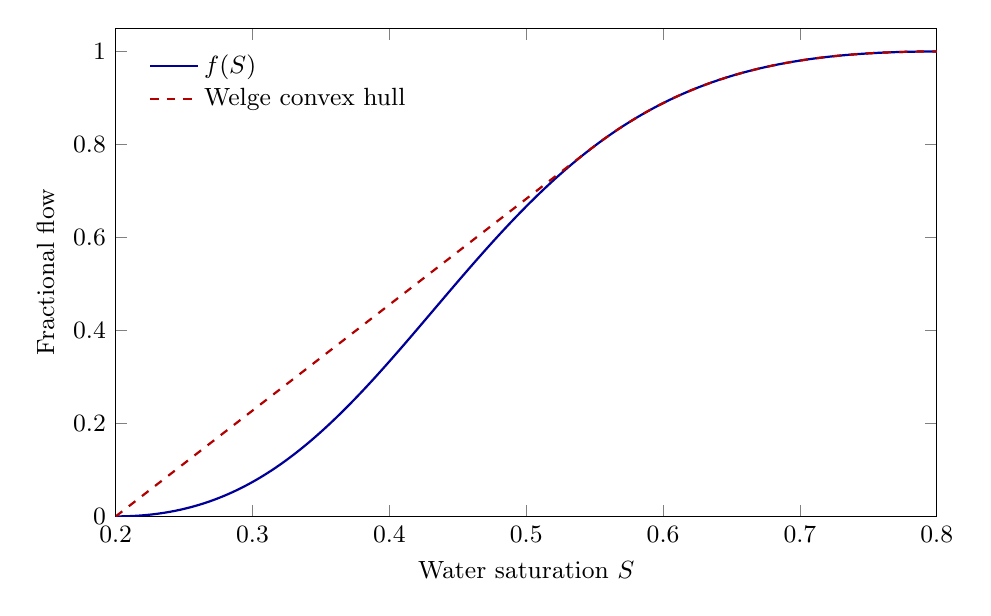
\begin{tikzpicture}
\begin{axis}[
  solveraxis,
  height=6.2cm,
  xlabel={Water saturation $S$},
  ylabel={Fractional flow},
  xmin=0.2, xmax=0.8,
  ymin=0, ymax=1.05,
  domain=0.2:0.8,
  samples=201,
  legend pos=north west,
]
\addplot[upwind] {ff(x)};
\addlegendentry{$f(S)$}
\addplot[welge] {hull(x)};
\addlegendentry{Welge convex hull}
\end{axis}
\end{tikzpicture}
\caption{Fractional flow for the default Corey data, with the Welge convex hull.
The hull is the tangent from $S_{wc}$ up to $S_f = 0.54641$, then $f$ itself.}
\label{fig:fflow}
\end{figure}

\section{Checks and a default run}

The process returns success only if all of the following hold.
\begin{center}
\begin{tabular}{@{}ll@{}}
\toprule
Check & Acceptance \\
\midrule
$\|f' - f'_{\mathrm{fd}}\|_\infty$ & $< 10^{-5}$ \\
Welge tangent residual & $< 10^{-6}$ \\
saturation $L_1$ against the Welge solution & $< 0.03$ \\
$\|p - p_{\mathrm{exact}}\|_\infty$ from~\eqref{eq:p-exact} & $< 10^{-6}$ \\
face flux against $1$ & $< 10^{-6}$ \\
conservation defect & $< 10^{-8}$ \\
\bottomrule
\end{tabular}
\end{center}
An $800$-cell release run ($t = 0.241577$ pore volumes, $\Delta t = 5.49\times 10^{-4}$, $440$ steps) produced
\begin{center}
\begin{tabular}{@{}lr@{}}
\toprule
Quantity & Value \\
\midrule
$S_f$, $v_s$, breakthrough & $0.54641$, $2.27671$, $0.43923$ \\
saturation $L_1$, $L_\infty$ & $0.00414$, $0.293$ \\
shock $x$, numerical / exact & $0.558$ / $0.550$ \\
pressure and face-flux errors & $3.6\times 10^{-11}$, $1.6\times 10^{-11}$ \\
conservation defect & $1.7\times 10^{-15}$ \\
inlet pressure, $t=0$ then $t_{\mathrm{end}}$ & $3.799$ then $4.008$ \\
pressure CG iterations, average & $12.4$ \\
transport BiCGStab iterations, average & $1$ \\
\bottomrule
\end{tabular}
\end{center}
The $L_\infty$ gap is the smeared shock: a first-order implicit upwind step cannot keep a discontinuity in one cell, while the Welge solution is sharp.
The $L_1$ error is the meaningful accuracy measure, and it is a few thousandths of a saturation unit.
The inlet pressure rises because $\lambda_t(S)$ for these Corey exponents has a minimum between $S_{wc}$ and $S_{\max}$.
The same rate then requires a larger drawdown.
The tight streak adds a steep segment to $p(x)$ on $[0.45, 0.55]$, shaded in Figure~\ref{fig:profile}.
The exact discrete pressure lies on the AMGCL curve.
The saturation plot is the same pair of curves the program writes to \texttt{output/profile.svg}.

\begin{figure}[ht]
\centering
\begin{tikzpicture}
\begin{axis}[
  solveraxis,
  height=5.4cm,
  xlabel={$x$},
  ylabel={Saturation $S$},
  xmin=0, xmax=1,
  ymin=0.15, ymax=0.86,
  legend pos=north east,
]
\addplot[upwind] table[x=x, y=S, col sep=comma] {profile.csv};
\addlegendentry{implicit upwind}
\addplot[welge] table[x=x, y=S_exact, col sep=comma] {profile.csv};
\addlegendentry{Welge}
\end{axis}
\end{tikzpicture}\\[1.2ex]
\begin{tikzpicture}
\begin{axis}[
  solveraxis,
  height=5.4cm,
  xlabel={$x$},
  ylabel={Pressure $p$},
  xmin=0, xmax=1,
  ymin=0, ymax=4.4,
  legend pos=north east,
]
\fill[black!8] (axis cs:0.45,0) rectangle (axis cs:0.55,4.4);
\addplot[upwind] table[x=x, y=p, col sep=comma] {profile.csv};
\addlegendentry{AMGCL}
\addplot[welge] table[x=x, y=p_exact, col sep=comma] {profile.csv};
\addlegendentry{exact discrete}
\end{axis}
\end{tikzpicture}
\caption{Default $800$-cell run at $t = 0.242$ pore volumes, from \texttt{profile.csv}.
Top: implicit upwind saturation and the Welge profile. The shock is spread over a few cells.
Bottom: pressure. The shaded band is the streak $k = 0.1$.}
\label{fig:profile}
\end{figure}

\section{Build and output}

AMGCL~1.4.3 is the Git submodule \texttt{third\_party/amgcl}. The repository records that release commit; \texttt{.gitmodules} only names the URL.
Clone the project and that submodule together:
\begin{lstlisting}
git clone --recurse-submodules ^
  https://github.com/konkolchin/buckley-leverett-amgcl.git
\end{lstlisting}
If the project is already present and \texttt{third\_party/amgcl} is empty, fetch the recorded commit with
\begin{lstlisting}
git submodule update --init
\end{lstlisting}
From a Visual Studio~2022 x64 developer prompt, in the project directory,
\begin{lstlisting}
cmake -S . -B build -G "Visual Studio 17 2022" -A x64
cmake --build build --config Release
build\Release\buckley.exe
\end{lstlisting}
The executable writes \texttt{output/}:
\begin{center}
\begin{tabular}{@{}ll@{}}
\toprule
File & Contents \\
\midrule
\texttt{report.txt} & AMG hierarchies, iteration counts, errors \\
\texttt{profile.csv} & $x$, $S$, Welge $S$, $p$, exact discrete $p$, $k$, $\lambda_t$, $f$ \\
\texttt{fractional\_flow.csv} & $S$, $k_{rw}$, $k_{ro}$, $f$, convex hull \\
\texttt{profile.svg} & saturation against Welge, and the pressure profile \\
\bottomrule
\end{tabular}
\end{center}

The program is a study solver for the classical one-dimensional waterflood.
The AMGCL calls are the real library interface: \texttt{make\_solver}, smoothed aggregation, SPAI(0), ILU(0), CG, and BiCGStab, with a CRS tuple as the matrix.
It is not a multi-well black-oil simulator, and it does not exercise CPR.

\end{document}
